\section{Pivoting and the price of a dense pair}
\label{pivot:sec:pivots}

Throughout this Section, $p$ is the price function of
\cref{thm:prices}, under the assumption that no finite win exists.
By \cref{price:word-bounds}, identity padding does not change price,
every nontrivial elementary coordinate shear has price one, and
every invertible two-coordinate matrix has price at most two.

\subsection{A general pivot inequality}

\begin{samepage}
\begin{lemma}[Pivot inequality]\label{lem:pivot-bound}
Let
\[
 K=\begin{pmatrix}A&C\\ B&D\end{pmatrix}\in\GL_{n+r}(\C),
 \qquad A\in\GL_n(\C),\quad D\in\GL_r(\C).
\]
Write the action of $K$ as
$(x,z_{\rm in})\mapsto(x',z_{\rm out})$.
The map $(x,z_{\rm out})\mapsto(x',z_{\rm in})$ is the invertible matrix
\begin{equation}\label{pivot:eq:pivot-matrix}
 \widetilde K=
 \begin{pmatrix}
 A-CD^{-1}B&CD^{-1}\\
 -D^{-1}B&D^{-1}
 \end{pmatrix},
 \qquad p(\widetilde K)\le p(K)+4r.
\end{equation}
\end{lemma}
\end{samepage}

\begin{proof}
Solving $z_{\rm out}=Bx+Dz_{\rm in}$ gives the displayed formula.
Its determinant is $\det A/\det D$, as follows by taking the Schur
complement of $D^{-1}$, so it is invertible. Both pivot hypotheses
are relevant: $D$ makes the solve possible, whereas $A$ makes its
resulting transition invertible.

We realize this solve as a feedback operation to which
\cref{thm:feedback} applies. Use data $(x,y)$ of widths $n,r$ and
state $z$ of width $r$. First apply, separately on the $r$ pairs
$(y_i,z_i)$, the matrix
\[
 P_\beta=\begin{pmatrix}\beta&1\\1&1\end{pmatrix},
 \qquad (\widehat y,z_{\rm in})=(\beta y+z,y+z).
\]
Next apply $K$ on $(x,z_{\rm in})$, leaving $\widehat y$ fixed.
Finally apply
\[
 Q_\beta=\begin{pmatrix}1&1-\beta\\1&-\beta\end{pmatrix}
 \quad\hbox{on each pair }(\widehat y_i,z_{{\rm out},i}),
\]
with outputs $(y',z')$. The full cell, denoted $\mathcal K_\beta$,
sends $(x,y,z)$ to $(x',y',z')$. Since
$\det P_\beta=\beta-1$ and $\det Q_\beta=-1$, it is invertible
whenever $\beta\ne1$, and
\begin{equation}\label{pivot:eq:cell-price}
 p(\mathcal K_\beta)\le p(K)+4r.
\end{equation}
The blocks of this cell with respect to its data/state split are
\begin{equation}\label{pivot:eq:beta-cell}
 \mathcal K_\beta=
 \left(
 \begin{array}{cc|c}
 A&C&C\\
 (1-\beta)B&\beta\Id_r+(1-\beta)D&\Id_r+(1-\beta)D\\ \hline
 -\beta B&\beta(\Id_r-D)&\Id_r-\beta D
 \end{array}
 \right).
\end{equation}
Its direct data block
\[
 M_\beta=
 \begin{pmatrix}A&C\\(1-\beta)B&\beta\Id_r+(1-\beta)D\end{pmatrix}
\]
has polynomial determinant and satisfies $M_0=K$. Thus the precise
genericity requirement is
\begin{equation}\label{pivot:eq:beta-exceptions}
 \beta\notin\{0,1\}\cup
 \{b\in\C:\det M_b=0\}.
\end{equation}
This excludes only finitely many numbers and hence allows a choice of
$\beta$. At feedback parameter one, the feedback denominator is
$\Id_r-(\Id_r-\beta D)=\beta D$, which is invertible.

Indeed, closing the state by $z=z'$ in
$z'=\beta y+z-\beta z_{\rm out}$ forces
$z_{\rm out}=y$. Consequently
\[
 y'=\beta y+z+(1-\beta)z_{\rm out}=y+z=z_{\rm in}.
\]
The feedback output map on $(x,y)$ is therefore exactly
$\widetilde K$, already proved invertible. The full cell, its direct
block, its feedback denominator, and its output all meet the hypotheses
of \cref{thm:feedback}. That Theorem and
\cref{pivot:eq:cell-price} prove the inequality.
\end{proof}

An empty data block gives $\widetilde K=D^{-1}$ and the inequality
directly from inverse symmetry. An empty pivot block makes no change.
We use these conventions if either block has width zero.

\subsection{One shared coordinate and exact scalar pivots}

\begin{lemma}[One-coordinate intersection]\label{pivot:lem:one-port}
Suppose a call to $Y_1\in\GL_a(\C)$ is followed by a call to
$Y_2\in\GL_b(\C)$, and their ordered coordinate sets intersect in
exactly one coordinate. If $P$ is their product on the union of these
sets, then
\[
 p(P)=p(Y_1)+p(Y_2).
\]
The same equality holds with any additional identity coordinates.
\end{lemma}

\begin{proof}
Let the shared coordinate occupy port $i_0$ of $Y_1$ and port $j_0$
of $Y_2$. Index the tensor grid by
$(i,j)\in\{1,\ldots,a\}\times\{1,\ldots,b\}$.
The usual word for $Y_1\otimes Y_2$ first applies $Y_1$ along each
fiber with fixed $j$, and then $Y_2$ along each fiber with fixed $i$.
Calls within either stage have disjoint coordinate sets, so put the
$j=j_0$ call last in the first stage and the $i=i_0$ call first in the
second stage. These two consecutive calls have the prescribed port
identification: send port $i$ of $Y_1$ to $(i,j_0)$ and port $j$ of
$Y_2$ to $(i_0,j)$.
\Cref{pivot:fig:tensor-grid} shows the selected fibers of this
consecutive call pair and their single shared coordinate.

Their union has $a+b-1$ coordinates. On all other grid coordinates
their product is identity, so the consecutive subproduct is a
permutation conjugate of
\[
 P\oplus\Id_{ab-(a+b-1)}
   =P\oplus\Id_{(a-1)(b-1)}.
\]
The exact direct-sum law makes its price $p(P)$, even when this padding
is empty. Grouping these two calls in the tensor word yields
\[
 b\,p(Y_1)+a\,p(Y_2)
 =p(Y_1\otimes Y_2)
 \le (b-1)p(Y_1)+(a-1)p(Y_2)+p(P).
\]
Thus $p(P)\ge p(Y_1)+p(Y_2)$. Product subadditivity applied to the
two identity-padded calls gives the reverse inequality.
\end{proof}

\begin{figure}[htbp]
\centering
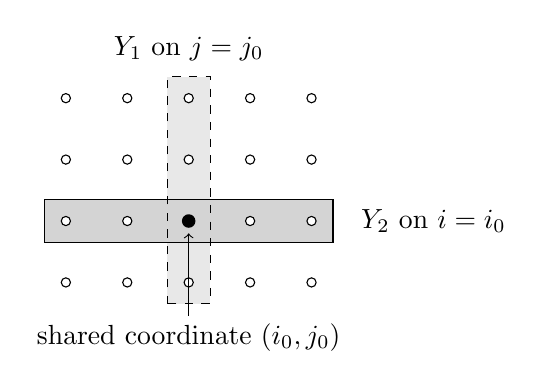
\begin{tikzpicture}[scale=.78]
 \fill[black!9] (2.65,.65) rectangle (3.35,4.35);
 \fill[black!17] (.65,1.65) rectangle (5.35,2.35);
 \draw[dashed] (2.65,.65) rectangle (3.35,4.35);
 \draw (.65,1.65) rectangle (5.35,2.35);
 \foreach \i in {1,...,4} {
   \foreach \j in {1,...,5} {
     \fill[white] (\j,\i) circle (.075);
     \draw (\j,\i) circle (.075);
   }
 }
 \fill (3,2) circle (.11);
 \node at (3,4.8) {$Y_1$ on $j=j_0$};
 \node[anchor=west] at (5.65,2) {$Y_2$ on $i=i_0$};
 \node at (3,.1) {shared coordinate $(i_0,j_0)$};
 \draw[->] (3,.45)--(3,1.8);
\end{tikzpicture}
\caption{The selected tensor fibers share exactly one coordinate.
Their two-call product fixes the $(a-1)(b-1)$ coordinates outside
the cross. Other calls of the tensor word occur before or after this
consecutive pair.}
\label{pivot:fig:tensor-grid}
\end{figure}

\begin{lemma}[Scalar pivot invariance]\label{lem:scalar-pivot}
Under the hypotheses of \cref{lem:pivot-bound}, if $r=1$, then
$p(\widetilde K)=p(K)$.
\end{lemma}

\begin{proof}
Write $D=d\ne0$. For each positive integer $\ell$, use $\ell$
copies of $K$, with fresh data groups $x_1,\ldots,x_\ell$ of width
$n$ and one shared state coordinate. In chronological order the
recurrences are
\begin{equation}\label{pivot:eq:chain-forward}
 y_j=Ax_j+Cw_{j-1},\qquad
 w_j=Bx_j+dw_{j-1},\qquad 1\le j\le\ell.
\end{equation}
Let $\mathcal C_\ell$ send
$(x_1,\ldots,x_\ell,w_0)$ to
$(y_1,\ldots,y_\ell,w_\ell)$. At every extension the previous
chain is regarded as a matrix only on its old data groups and its
one state coordinate. The next data group is outside this set, so
the intersection with the next call is exactly the one state
coordinate. Coordinates fixed by the old chain remain members of
its old set; no padding from the tensor-grid proof is added to it.
Induction using \cref{pivot:lem:one-port} gives
\begin{equation}\label{pivot:eq:forward-chain-price}
 p(\mathcal C_\ell)=\ell p(K).
\end{equation}

The full chain is invertible as a product of invertible calls. Its
state-to-state block is $d^\ell$, and its direct block on the data is
lower block triangular with diagonal blocks $A$. In fact its
$(j,i)$ block for $i<j$ is $Cd^{j-1-i}B$, and its blocks for $i>j$
vanish. Both blocks required by \cref{lem:pivot-bound} are therefore
invertible for every $\ell$.

Pivoting the boundary state means that $w_\ell$ is given and $w_0$
is requested. The exact backward recurrence is
\begin{equation}\label{pivot:eq:chain-backward}
 w_{j-1}=d^{-1}w_j-d^{-1}Bx_j,\qquad
 y_j=(A-Cd^{-1}B)x_j+Cd^{-1}w_j.
\end{equation}
Thus the pivoted chain $\widetilde{\mathcal C}_\ell$ consists of
copies of $\widetilde K$ in the order $j=\ell,\ldots,1$, again
with fresh data groups and one shared state. The same intersection
argument gives
\begin{equation}\label{pivot:eq:reverse-chain-price}
 p(\widetilde{\mathcal C}_\ell)=\ell p(\widetilde K).
\end{equation}
Put $S=A-Cd^{-1}B$. Since $\det K=d\det S$, the matrix $S$ is
invertible. The reverse chain has state block $d^{-\ell}$ and a
direct data block upper triangular in chronological order, with
diagonal blocks $S$; equivalently it is lower triangular in reverse
chronological order. Its full matrix is invertible too. Hence
\cref{lem:pivot-bound} applies both to the forward chain and to
the reverse chain. Pivoting the reverse chain returns the forward
chain, and therefore
\[
 \ell p(\widetilde K)\le\ell p(K)+4,
 \qquad
 \ell p(K)\le\ell p(\widetilde K)+4.
\]
Equivalently, $|p(\widetilde K)-p(K)|\le4/\ell$ for every $\ell$.
Letting $\ell$ tend to infinity proves equality. The earlier pivot
inequality is an exact statement for each finite matrix, so this
argument requires no estimate uniform in the increasing data width.
\end{proof}

\begin{corollary}[Exchange of two basis members]
\label{pivot:cor:basis-exchange}
Let $U=(u_1,\ldots,u_n,u_*)$ and
$V=(v_1,\ldots,v_n,v_*)$ be ordered bases of the same space of
linear forms, viewing each list as a column vector of its forms, and let
\[
 V=KU,\qquad K=\begin{pmatrix}A&C\\B&d\end{pmatrix}.
\]
The exchanged lists
\[
 U'=(u_1,\ldots,u_n,v_*),\qquad
 V'=(v_1,\ldots,v_n,u_*)
\]
are both bases if and only if $d\ne0$ and $\det A\ne0$.
Whenever this holds, the transitions $U\mapsto V$ and
$U'\mapsto V'$ have equal price. The statement applies to any
chosen member of each basis after reordering them to the last
positions.
\end{corollary}

\begin{proof}
Relative to $U$, the coefficient matrices of $U'$ and $V'$ are
\[
 \begin{pmatrix}\Id_n&0\\ B&d\end{pmatrix},\qquad
 \begin{pmatrix}A&C\\0&1\end{pmatrix},
\]
with determinants $d$ and $\det A$, respectively. These give the
asserted criterion exactly. When both are nonzero, the transition
between them is \cref{pivot:eq:pivot-matrix} with scalar pivot.
Apply \cref{lem:scalar-pivot}. Reorderings have zero price.
\end{proof}

\subsection{Four forms and the dense-pair bound}

\begin{lemma}[Price of a dense pair]\label{lem:pair-price}
Every invertible $2\times2$ matrix all of whose entries are nonzero
has price at most $3/2$. In particular,
\begin{equation}\label{pivot:eq:pair-bound}
 p\left(\begin{pmatrix}1&1\\1&u\end{pmatrix}\right)
 \le\frac32\qquad (u\in\C\setminus\{0,1\}).
\end{equation}
\end{lemma}

\begin{proof}
For a pair matrix $H$, the tensor law reads
$p(H\otimes H)=4p(H)$. We therefore seek a four-coordinate map
of price at most six that becomes a tensor square after monomial
changes. Two shears and the basis exchanges below put this map into
the form of a rank-one perturbation of the identity, making the
required monomial changes explicit.

Fix $\lambda\in\C\setminus\{0,1\}$ and four independent linear
forms $a,b,c,d$. We first bound the transition from
\[
 Y^{(0)}=(a,b,c,d)\quad\hbox{to}\quad
 X=(a+b,b+c,c+d,d+\lambda a).
\]
Its matrix is $\Id_4+J$, where
\[
 J=\begin{pmatrix}
 0&1&0&0\\0&0&1&0\\0&0&0&1\\\lambda&0&0&0
 \end{pmatrix},\qquad J^4=\lambda\Id_4.
\]
Here $J$ is monomial because $\lambda\ne0$, and
\[
 (\Id_4+J)(\Id_4-J+J^2-J^3)=(1-\lambda)\Id_4
\]
shows that $\Id_4+J$ is invertible. Apply
\cref{thm:feedback} at parameter one to
\[
 \mathcal L=\begin{pmatrix}\Id_4&J\\\Id_4&0\end{pmatrix}.
\]
This full cell is invertible, its direct block and feedback
denominator are identities, and its output is $\Id_4+J$.
To implement $\mathcal L$, send $(h,l)$ to $(h,Jl)$ by a monomial,
add $h_i$ into the second coordinate of each of the four pairs,
and swap the two blocks. Consequently
\begin{equation}\label{pivot:eq:four-start}
 p(\Id_4+J)\le p(\mathcal L)\le4.
\end{equation}

We change the first and third members on the $Y$ side using two
shears and legal exchanges. For clarity, all intermediate lists
are displayed below. Put
\[
 X_b=(a+b,b,c+d,d+\lambda a),\qquad
 X_d=(a+b,b+c,c+d,d).
\]
Every determinant in the last two columns is computed from the
coefficient rows in the original ordered basis $(a,b,c,d)$.
\begin{center}
\small
\begin{tabular}{@{}c l c c c@{}}
\toprule
Stage & $Y$ list & $X$ list & $\det Y$ & $\det X$\\
\midrule
0 & $(a,b,c,d)$ & $X$ & $1$ & $1-\lambda$\\
1 & $(a,b+c,c,d)$ & $X_b$ & $1$ & $1$\\
2 & $(a+b+c,b+c,c,d)$ & $X_b$ & $1$ & $1$\\
3 & $(a+b+c,b,c,d)$ & $X$ & $1$ & $1-\lambda$\\
4 & $(a+b+c,b,c,d+\lambda a)$ & $X_d$ & $1$ & $1$\\
5 & $(a+b+c,b,c+d+\lambda a,d+\lambda a)$
  & $X_d$ & $1$ & $1$\\
6 & $(a+b+c,b,c+d+\lambda a,d)$
  & $X$ & $1-\lambda$ & $1-\lambda$\\
\bottomrule
\end{tabular}
\end{center}
The steps $0\to1$ and $2\to3$ exchange the second members;
the steps $3\to4$ and $5\to6$ exchange the fourth members.
The step $1\to2$ adds the second member of $Y$ into its first,
and $4\to5$ adds its fourth member into its third. These are
the only two shears. The determinant table proves that every list
is a basis, including on both sides of every exchange; it follows
also by direct elementary row operations. Thus
\cref{pivot:cor:basis-exchange} applies at all four exchanges.
Changing the source basis from $Y$ to $EY$ by a shear replaces its
transition matrix $T$ by $TE^{-1}$, increasing price by at most one.
Together with \cref{pivot:eq:four-start}, this proves that the
transition from the last $Y$ list to $X$ has price at most six.

Reorder these final lists as
\[
 \overline Y=(a+b+c,b,d,c+d+\lambda a),\qquad
 \overline X=(b+c,b+a,d+\lambda a,c+d).
\]
Let
\[
 k=(1,-1,1,-1)^{\mathsf T},\qquad
 \Delta=(-1,1,\lambda,-\lambda)^{\mathsf T}.
\]
Then $k^{\mathsf T}\overline Y=(1-\lambda)a$ and
$\overline X-\overline Y=\Delta a$, so the transition matrix is
the explicit rank-one perturbation
\begin{equation}\label{pivot:eq:rank-one}
 T=\Id_4+\frac{\Delta k^{\mathsf T}}{1-\lambda},
 \qquad p(T)\le6.
\end{equation}

We now give the diagonal scalings. All their entries are nonzero
under the stated hypotheses on $\lambda$. Set $u=\lambda^{-1}$ and
\[
 L_1=\diag\left(\frac{1-\lambda}{\Delta_1},
 \frac{1-\lambda}{\Delta_2},
 \frac{1-\lambda}{\Delta_3},
 \frac{1-\lambda}{\Delta_4}\right),\qquad
 R_1=\diag(1,-1,1,-1).
\]
The rank-one summand of $L_1TR_1$ has every entry equal to one,
and a direct calculation gives
\[
 L_1TR_1=
 \begin{pmatrix}
 \lambda&1&1&1\\1&\lambda&1&1\\
 1&1&u&1\\1&1&1&u
 \end{pmatrix}.
\]
With the further scalings
\[
 L_2=\diag(u,u,u,1),\qquad R_2=\diag(1,1,1,\lambda),
\]
we obtain
\begin{equation}\label{pivot:eq:tensor-rescaling}
 L_2L_1TR_1R_2=
 \begin{pmatrix}
 1&u&u&1\\u&1&u&1\\u&u&u^2&1\\1&1&1&1
 \end{pmatrix}.
\end{equation}
Write $B(u)=\left(\begin{smallmatrix}1&1\\1&u\end{smallmatrix}\right)$.
The $(\alpha,\gamma)$ entry of $B(u)\otimes B(u)$, for bit pairs
$\alpha,\gamma\in\{0,1\}^2$, is
$u^{\alpha_1\gamma_1+\alpha_2\gamma_2}$.
Ordering its rows by $10,01,11,00$ and its columns by
$01,10,11,00$ gives exactly \cref{pivot:eq:tensor-rescaling}.
All the scalings and permutations preserve price. The tensor law
therefore yields
\[
 4p(B(u))=p(B(u)\otimes B(u))=p(T)\le6.
\]
Every $u\ne0,1$ arises from the permitted choice $\lambda=1/u$,
proving \cref{pivot:eq:pair-bound}.

Finally, if $H=\left(\begin{smallmatrix}a&b\\c&d\end{smallmatrix}\right)$
is dense and invertible, then
\[
 \diag(a^{-1},c^{-1})\,H\,\diag(1,a/b)
 =B\left(\frac{ad}{bc}\right).
\]
Density makes $ad/(bc)\ne0$, and invertibility makes it different
from one. Monomial invariance completes the proof.
\end{proof}
